%\clearpage
\chapter{Etat de l'art}
\label{sec:SOTA}

Dans le cadre de cette thèse, nous cherchons dans un premier temps à lier la dynamique des articulations d'un piéton à une intention. Cette estimation de la dynamique des articulations sera ensuite combinée à la vision afin d’avoir une estimation plus robuste et absolue de l'intention du piéton en fonction de son environnement.\\

L'idée de restreindre la gestuelle d'une personne à la seule dynamique de son ossature n'est pas nouvelle.
Durant les années 70, les travaux en psychologie de Johansson  \cite{johansson1973visual,johansson1976spatio} ont permis de montrer qu'avec seulement des points lumineux, l'être humain interprétait facilement les stimulis qui lui étaient présentés comme ceux d'un être humain effectuant des actions: l'humain peut donc reconnaitre une action juste avec la pose et sans information annexe telle que l'environnement. 

De ce fait, nous avons souhaité voir s'il était possible de réaliser l'analogie entre les travaux réalisés sur le stimuli humain et la machine.

\begin{figure}[H]
    \centering
    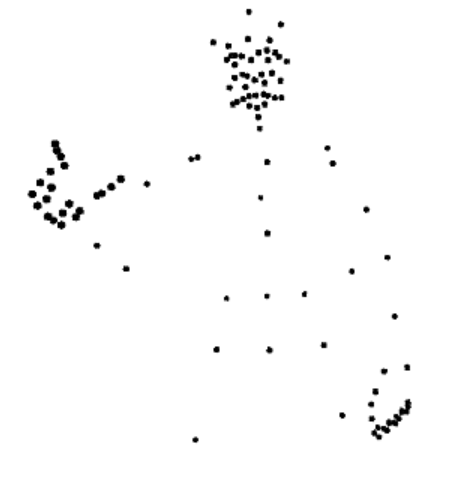
\includegraphics[width=0.34\linewidth]{Images/Johansson.png}
    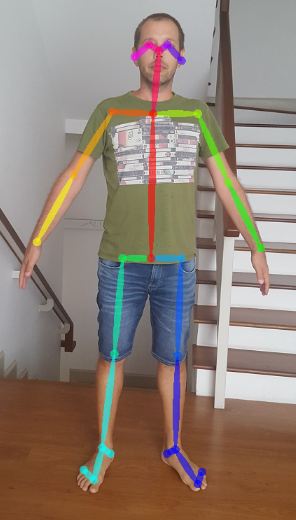
\includegraphics[width=0.2\linewidth]{Images/openpose2.png}
    \caption{A gauche: Un exemple de stimuli de l'experience de Johansson \cite{johansson1973visual,johansson1976spatio}.\\ A droite: la squelettisation obtenue après l'application d'Openpose \cite{cao2017realtime}}
    \label{fig:Johansson}
\end{figure}

\textit{De ce fait, nous avons du nous intérésser à plusieurs étapes qui seront considérées comme des parties indépendantes de notre approche}


PipeLine: SQUELETTE -> HAR -> INTENTION

\section{Squelettisation de piétons}

Afin d’aboutir à cet objectif, la première étape essentielle est la détection des piétons. De nombreuses méthodes existent dans l’état de l’art, notamment par apprentissage profond où les récents résultats sont tout à fait prometteurs. La méthode finale ciblée concernant la prédiction des intentions raisonne sur la posture des piétons et nécessite donc d’être à même d’effectuer une extraction des articulations majeures des piétons en temps réel pour ensuite alimenter la phase de prédiction.

La tâche de détection est compliquée par la variabilité de l’apparence des personnes (vêtements, pose ...)
ainsi que par des phénomènes d’occlusions, dûs à la foule et au décor ou encore dûs à des problèmes d'echelle dans l'image.

%https://nanonets.com/blog/human-pose-estimation-2d-guide/?utm_source=reddit&utm_medium=social&utm_campaign=pose&utm_content=GROUP_NAME


\label{subsec:SQUEL}
\subsection{Approches Top Down}
\subsection{Approches Bottom Up}

\section{Human Action Recognition}
\label{subsec:HAR}

La seconde étape de l'approche consistera en la classification des actions de la personne. La reconnaissance de l'action humaine dans une vidéo est un sujet de recherche difficile de par la grande variation et la complexité des données en entrée.

Les principales modalités utilisées pour la reconnaissance d'actions humaines comprennent les vidéos RGB dans leur intégralité \cite{donahue2015long,2014arXiv1412.0767T,varol2017long,Wu_2018_CVPR}, le flow optique \cite{simonyan2014two,zhang2016real,sevilla2018integration,DanutPOP} et la réprésentation sous forme de squelette \cite{vemulapalli2014human,du2015hierarchical,2016arXiv160707043L,2018arXiv180107455Y}.

Selon notre problématique: lier la dynamique de la pose à une classe, nous nous sommes majoritairement intéréssés à la dernière famille d'approches. La représentation sous forme de squelette qui semble être l'approche la plus robuste mais également la plus plausible pour une utilisation en temps réel:

\begin{itemize}
    \item En réduisant la taille des données d'entrée grâce à la structure de données associée aux squelettes, ce type d'approche est considéré comme bien plus rapide computationellement parlant que les modalitées listées précédement.
    \item Par ailleurs, celles-ci sont généralement bien plus robustes et capables de représenter les informations invarriantes d'une action puisque qu'aucun contexte de fond n'y est inclus.
\end{itemize}

pb spatio temporel -> comment le traiter?

\subsection{Approches récurrentes}

Ces dernières années, les réseaux de neurones récurrents ont  été les approches de référence pour la modélisation de séquences en matière de reconnaissance vocale, de traitement numérique des signaux, de traitement vidéo et d'analyse des données textuelles. 


Analogiquement, la plupart des approches d'apprentissage profond pour la reconnaissance de gestes utilisent également des cellules récurrentes type LSTM \cite{hochreiter1997long} ou GRU \cite{2014arXiv1406.1078C}.

On représente le squelette sous forme d’une séquence et on y applique des réseaux de neurones à état, permettant de conserver l’information d’un instant de la séquence à un autre.

Ainsi, Baccouche et\textit{ al.}\cite{baccouche2011sequential} proposent une architecture combinant LSTM et RNN pour la reconnaissance d'actions.
Avola et\textit{ al.} \cite{avola2018exploiting} exploitent les caractéristiques des angles de jointures apprises grâce à une architecture de type LSTM. 
Zhang et\textit{ al.}\cite{zhang2017geometric} génèrent à partir des articulations, huit indicateurs géométriques et les évaluent avec un réseau LSTM à trois couches.
Du et\textit{ al.}\cite{du2015hierarchical} divisent le squelette humain en cinq parties puis proposent une approche hierarchique séquentielle.
Shukla et\textit{ al.}\cite{shukla2017recurrent} proposent une architecture récurente hierarchique sensiblement équivalente à \cite{du2015hierarchical} mais réduisent le nombre de jointures en entrée du modèle, certaines étant considérées comme superflues et ne portant que peu d'information. Conduisant à un ensemble réduit de paramètres, diminuant le temps d'inférence sans dégrader la qualité du classificateur.
Shahroudy et\textit{ al.}\cite{shahroudy2016ntu} utilisent une approche LSTM se basant sur un apprentissage à long terme des cooccurrences d'articulations caractérisant intrinsèquement les actions humaines.
Zhang et\textit{ al.}\cite{zhang2017view} proposent un réseau récurrent adaptatif avec une architecture LSTM, permettant au réseau de s'adapter aux points de vue d'observation les plus appropriés de bout en bout afin de gérer les grandes variations d'orientation dans les actions.

 

\subsection{Approches convolutives}
Les cellules récurrentes étant relativement lentes et difficiles à entrainer ainsi qu'à utiliser en temps réel comparé aux approches dites convolutives, celles-ci sont alors devenues une solution intéressante compte tenu de leurs avantages en matière de parallélisation, d'efficacité dans l'apprentissage des caractéristiques et de rapidité.


Les approches convolutives peuvent par exemple représenter le squelette sous la forme d'une pseudo-image pour appliquer des convolutions 2D, ou tout autre version spatio-temporelle des CNN comme les convolutions 3D: les données squelettiques sont des éléments de faible dimension. Il est donc naturel d'organiser une séquence de caractéristiques du squelette de manière chronologique dans une image, qui conserve les informations originales de la dynamique du squelette.

\begin{figure}[H]
    \centering
    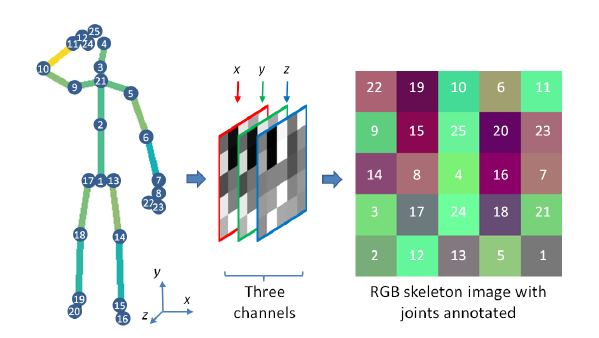
\includegraphics[width=0.7\linewidth]{Images/skeltoim.png}
    \caption{Organisation de la structure de données squelette en 3D en une image à trois channel (RGB)}
    \label{fig:skeltoim}
\end{figure}
L’idée étant d’utiliser la connaissance du domaine image qui s’est améliorée ces dernière années et de structurer les données pour leur donner la forme escomptée (une suite d’image) et enfin réaliser une classification habituelle.

Ainsi, Ke \textit{et\textit{ al.}}(2017) \cite{ke2017new} proposent de transformer une séquence squelette sous la forme de clips vidéos

to transform a skeleton
sequence to three video clips for robust feature learning
and action recognition. We proposed to use a pre-trained
CNN model followed by a temporal pooling layer to extract
a compact representation of each frame. The CNN features
of the three clips at the same time-step are concatenated in
a single feature vector,

Cao et\textit{ al.}\cite{cao2018skeleton}


En s'éloignant un peu plus du domaine image mais en conservant la notion de convolution, d'autres approches à base de CNN, les utilisent en tant que CNN 1D: 

Les réseaux récurrents et les réseaux convolutifs peuvent également être fusionnés. L'approche consiste à extraire les caractéristiques avec des couches convolutives, adaptées pour exploiter les informations spatiales, puis de modéliser la dynamique temporelle par des couches récurrentes.

Ainsi, Donahue et\textit{ al.} (2015) \cite{donahue2015long} proposent 

Li et\textit{ al.}(2017)\cite{li2017skeleton} proposent une approche où LSTM et CNN sont fusionnés "tardivement" (late fusion). Ullah et\textit{ al.}(2017)\cite{ullah2017action} proposent un approche bidirectionnelle où, les features obtenus par le CNN sont envoyés dans un LSTM bidirectionnel \cite{Schuster97bidirectionalrecurrent}, connectant deux couches cachées de directions opposées à la même sortie. La couche de sortie pouvant alors obtenir simultanément des informations sur les états passés et futurs.



\subsection{Attention}

Maghoumi et\textit{ al.}\cite{maghoumi2019deepgru} proposent des unités GRU empilées et un mécanisme d'attention globale ainsi que deux couches entièrement connectées.

\subsection{Graph Based}

\section{Intention Prediction}
\textit{La plupart des approches actuelles de la prédiction de l'action des piétons sont basées sur la trajectoire [16, 1, 5], ce qui signifie qu'elles s'appuient sur le mouvement passé observé des piétons et/ou la dynamique des véhicules pour prédire l'emplacement futur des piétons. Ces approches sont toutefois efficaces lorsque les piétons traversent déjà laa rue ou sont sur le point de le faire, c'est-à-dire que ces algorithmes réagissent à une action déjà en cours au lieu de l'anticiper.}

Un remède aux inconvénients courants des algorithmes basés sur la trajectoire est d'anticiper l'action en estimant sa cause ou son intention non déviante.


In the literature various terms such as intention, actionand behavior are used to describe what the agent is doing or about to do in the scene. Here, we distinguish intention as the underlying state of mind which cannot be observed but can be inferred from the behavior. This is opposed toactions and, more generally, behaviors, i.e. observable ac-tions such as walking or crossing, for which there is groundtruth available.




\subsection{Handcrafted}
\subsection{Apprentissage profond}


